\documentclass[12pt]{article}
\usepackage{algo,fullpage,url,amssymb,epsfig,color,xspace,tikz,amsmath}
\usepackage{graphicx}
\usepackage{makecell}
\usepackage{float}
\usepackage[pdftitle={CS 486 Assignment 1},
pdfsubject={University of Waterloo, CS 486, Winter 2024},
pdfauthor={Arne Storjohann}]{hyperref}
\usepackage{algpseudocode,enumitem,calc,multicol}

\usepackage{listings}
\lstset{%
        language=C++,
        keepspaces=true,
        basicstyle=\small\ttfamily,
       commentstyle=\footnotesize\itshape{},
       identifierstyle=\slshape{},
       keywordstyle=\bfseries,
       numbers=left,
       numberstyle=\tiny{},
       numberblanklines=false,
       inputencoding={utf8},
       columns=fullflexible,
       basewidth=.5em,
        fontadjust=true,
        tabsize=3,
        emptylines=*1,
       breaklines,
       breakindent=30pt,
        prebreak=\smash{\raisebox{-.5ex}{\hbox{\tiny$\hookleftarrow$}}},
    escapeinside={//*}{\^^M} % Allow to set labels and the like in comments starting with //*
	}

\renewcommand{\thesubsection}{Problem \arabic{subsection}}

\begin{document}

\begin{center}
  {\Large\bf University of Waterloo}\\ \vspace{3mm}
  {\Large\bf CS 486, Winter 2024}\\ \vspace{2mm}
  {\Large\bf Assignment 1}\\ \vspace{3mm}
\end{center}

\definecolor{care}{rgb}{0,0,0}
\def\question#1{\item[\bf #1.]}
\def\part#1{\item[\bf #1)]}
\newcommand{\pc}[1]{\mbox{\textbf{#1}}} % pseudocode

%%%%%%%%%%%%%%%%%%%%%%%%%%%%%%%%%%%%%%%%%%%%%
\subsection{} 
\begin{enumerate}
\part{a} 
	The Euclidean distance to the destination is an admissible heuristic function because it never overestimates the actual shortest path cost, as the shortest possible path between two cities is the straight line (Euclidean) distance between them, thus the only possible case is the Euclidean distance equals or \textbf{underestimates} the shortest path cost.

\part{b} 
	The Euclidean distance to the destination is a consistent heuristic function because it satisfies the monotone restriction: \textbf{heuristic estimate of the path cost is always less than or equal to the actual cost}. As previously stated the Euclidean distance could only equals or \textbf{underestimates} the shortest path cost.
	%\textbf{$h(n) -h(n) \le cost(m,n)$ for every arc $<m,n>$}

\part{c} Decision Tree:
	\begin{figure}[H]
	\center
	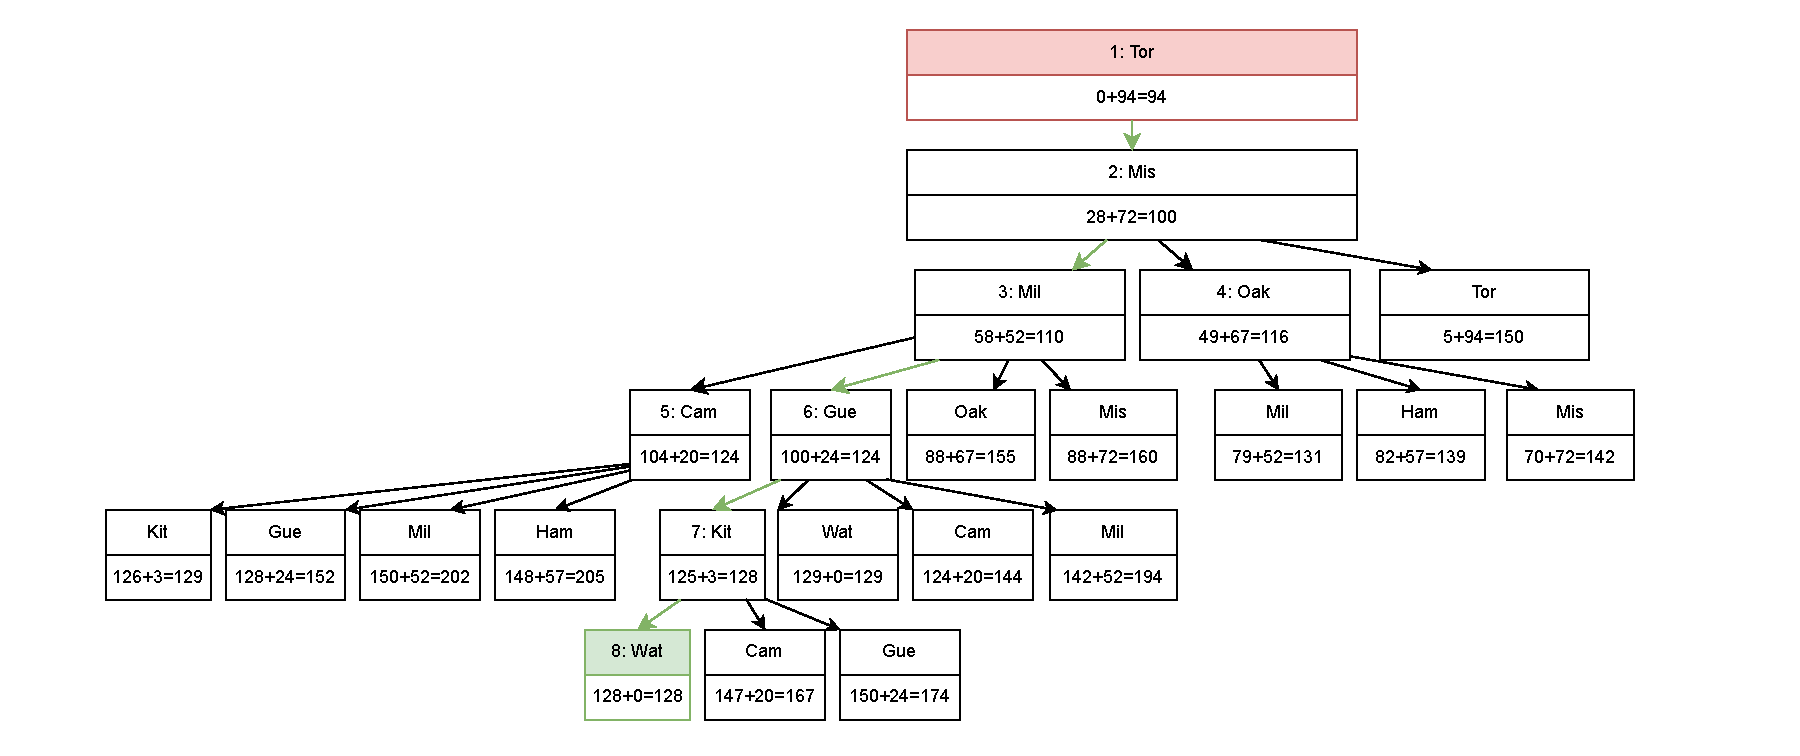
\includegraphics[width=12cm]{486A1Q1.pdf}
	\end{figure}

\end{enumerate}


%%%%%%%%%%%%%%%%%%%%%%%%%%%%%%%%%%%%%%%%%%%%%
%%%%%%%%%%%%%%%%%%%%%%%%%%%%%%%%%%%%%%%%%%%%%
\newpage
\subsection{} 
\begin{enumerate}
	
\part{b} 
	
	The game always terminates in less than 10 seconds (around \texttt{0.04s} to \texttt{0.05s}) on my laptop for \texttt{RandomPlayer} vs. \texttt{MinimaxHeuristicPlayer} with depth \texttt{2}.
	
	The first depth number i encountered for the game not terminating within 10 seconds is \texttt{depth=6}, which takes around \texttt{34s} on my Laptop.

\part{c} 

\part{d}

	\begin{tabular}{|c|c|c|c|c|}
	\hline
 	Agent 1 & Agent 2 & Wins & Draws & Losses \\
	\hline
	\makecell{Minimax Player, depth 3 \\ three\_line\_heur} & RandomPlayer & & & \\
	\hline
	\makecell{Minimax Player, depth 3 \\ my\_heuristic} & RandomPlayer & & & \\
	\hline
	\makecell{Minimax Player, depth 5 \\ three\_line\_heur} & \makecell{Minimax Player, depth 2 \\ three\_line\_heur} & & & \\
	\hline
 	\makecell{Minimax Player, depth 5 \\ my\_heuristic} & \makecell{Minimax Player, depth 2 \\ my\_heuristic} & & & \\
	\hline
	\makecell{Minimax Player, depth 5 \\ my\_heuristic} & \makecell{Minimax Player, depth 5 \\ three\_line\_heur} & & & \\
	\hline
	\end{tabular}

\end{enumerate}

%%%%%%%%%%%%%%%%%%%%%%%%%%%%%%%%%%%%%%%%%%%%%
%%%%%%%%%%%%%%%%%%%%%%%%%%%%%%%%%%%%%%%%%%%%%
\newpage
\subsection{} 
\begin{enumerate}
\part{1} 
	We will denote the $i$'th Queen's coordinate in the form $(X_i, Y_i)$. And the domain for them is $1 \le X_i \le N$ and $1 \le Y_i \le N$ for all $i \in \{1, 2, \dots, N\}$.
	
	And the constraints are:
	
	\begin{itemize}
		\item Row Constraint:
			$X_i \neq X_j $ for all  $i \neq j$ where $i,j \in \{1, 2, \dots, N\}$.
		
		\item Column Constraint:
			$Y_i \neq Y_j $ for all  $i \neq j$ where $i,j \in \{1, 2, \dots, N\}$.
			
		\item Diagonal Constraint: 
			$|X_i - X_j| \neq |Y_i - Y_j| $ for all  $i \neq j$ where $i,j \in \{1, 2, \dots, N\}$.

	\end{itemize}
		
\part{2} 
	We will denote the $i$'th Octopi's coordinate in the form $(X_i, Y_i)$. And the domain for them is $1 \le X_i \le N$ and $1 \le Y_i \le N$ for all $i \in \{1, 2, \dots, N\}$.
	
	And the constraints are:
	
	\begin{itemize}
		\item Row Constraint:
			$X_i \neq X_j $ for all  $i \neq j$ where $i,j \in \{1, 2, \dots, N\}$.
		
		\item Column Constraint:
			$Y_i \neq Y_j $ for all  $i \neq j$ where $i,j \in \{1, 2, \dots, N\}$.
			
		\item Block Constraint: 
			$\left\lfloor \frac{X_i - 1}{M} \right\rfloor \neq \left\lfloor \frac{X_j - 1}{M} \right\rfloor$ or $\left\lfloor \frac{Y_i - 1}{M} \right\rfloor \neq \left\lfloor \frac{Y_j - 1}{M} \right\rfloor$ for all  $i \neq j$ where $i,j \in \{1, 2, \dots, N\}$.


	\end{itemize}


\end{enumerate}

%%%%%%%%%%%%%%%%%%%%%%%%%%%%%%%%%%%%%%%%%%%%%
%%%%%%%%%%%%%%%%%%%%%%%%%%%%%%%%%%%%%%%%%%%%%

\end{document}
